\documentclass[12pt, a4paper]{article}
\usepackage[table]{xcolor} % Load the xcolor package with table option
\usepackage[utf8]{inputenc}
\usepackage[english]{babel}
\usepackage{times}
\usepackage{booktabs}
\usepackage{rotating}
\usepackage[margin=1in]{geometry}
\usepackage{fancyhdr}
\usepackage{amsmath}
\usepackage{graphicx}
\usepackage{amsmath}
\usepackage{geometry}
\usepackage{tabularx}
\usepackage{graphicx}
\usepackage{multirow}
\usepackage{xcolor}
\usepackage{hyperref}

\pagestyle{fancy}
\fancyhf{}
\renewcommand{\headrulewidth}{0pt}
% Title, author, and date
\title{CS3350B, Computer Organization\\
Assignment 4}
\author{}

\begin{document}

\maketitle
\thispagestyle{empty}


\section*{Submission Instructions}

\textcolor{purple}{
\paragraph{IMPORTANT} Before submitting your assignment, it is essential to check the following link: \href{https://bit.ly/3IJLx72}{https://bit.ly/3IJLx72}. This online document contains all clarifications and updates related to this assignment. The assignment PDF may undergo minor updates in certain circumstances. We ensure the most recent version of the assignment is always available in this link for download. To guarantee your submission is in line with the latest version of the assignment, always check this link before submitting.
}

\paragraph{Collaboration and Integrity Policy} For any question involving calculations, you must provide your workings. While collaboration with other students in the class on general strategies for solving the problems is permitted, each assignment and the answers within must be solely individual work and completed independently. Any form of plagiarism or the use of AI assistance, such as ChatGPT, will be taken seriously and may result in a mark of 0 on this assignment, removal from the course, or more severe consequences.


\paragraph{Single PDF Submission} All answers for this assignment must be submitted on OWL as a single PDF file, named ``asn4\_answer.pdf''. Failure to comply with this naming convention will result in a deduction of marks.

\paragraph{LaTeX Bonus} A bonus of up to 15\% of the total marks for this assignment (not exceeding the maximum mark) will be awarded for using the provided LaTeX template to complete the assignment. The template ensures a high level of readability and formatting consistency. The LaTeX file is provided as a .zip archive and is recommended to be uploaded to Overleaf for compilation into a PDF (you may also use other Latex compiler you like). You're encouraged to utilize the provided tables in the template for a more straightforward completion of your answers. Also, you may include additional figures as necessary. Remember, only the final PDF file needs to be submitted.

\paragraph{Other formart} While it is highly recommended to type your answers using the provided LaTeX template or another typing software, clear scans (not photographs) of handwritten work will be accepted if they are exceptionally legible. Please note that if your submission is difficult to read or interpret, it may be marked incorrect, with no option for re-evaluation.


\vfill
\hfill Copyright \textcopyright\ 2024 by CS3350 TAs

\newpage

\section*{Exercise}
\paragraph{Exercise 1. [10 Marks]} Consider the multi-cycle MIPS datapath presented in Figure~\ref{fig:cpu_big}, it shows 4 inter-stage registers: IF/ID, ID/EX, EX/MEM, and MEM/WB. Consider also the control signals presented in the diagram in blue. Assume the ALUOp control signal is 3 bits. Ignore control signals not shown (i.e. the ones controlling forwarding). Determine the minimum size, in bits, of each of the four inter-stage registers. For part marks, ensure to include workings and not just the total values.

\begin{figure}[h]
  \centering
  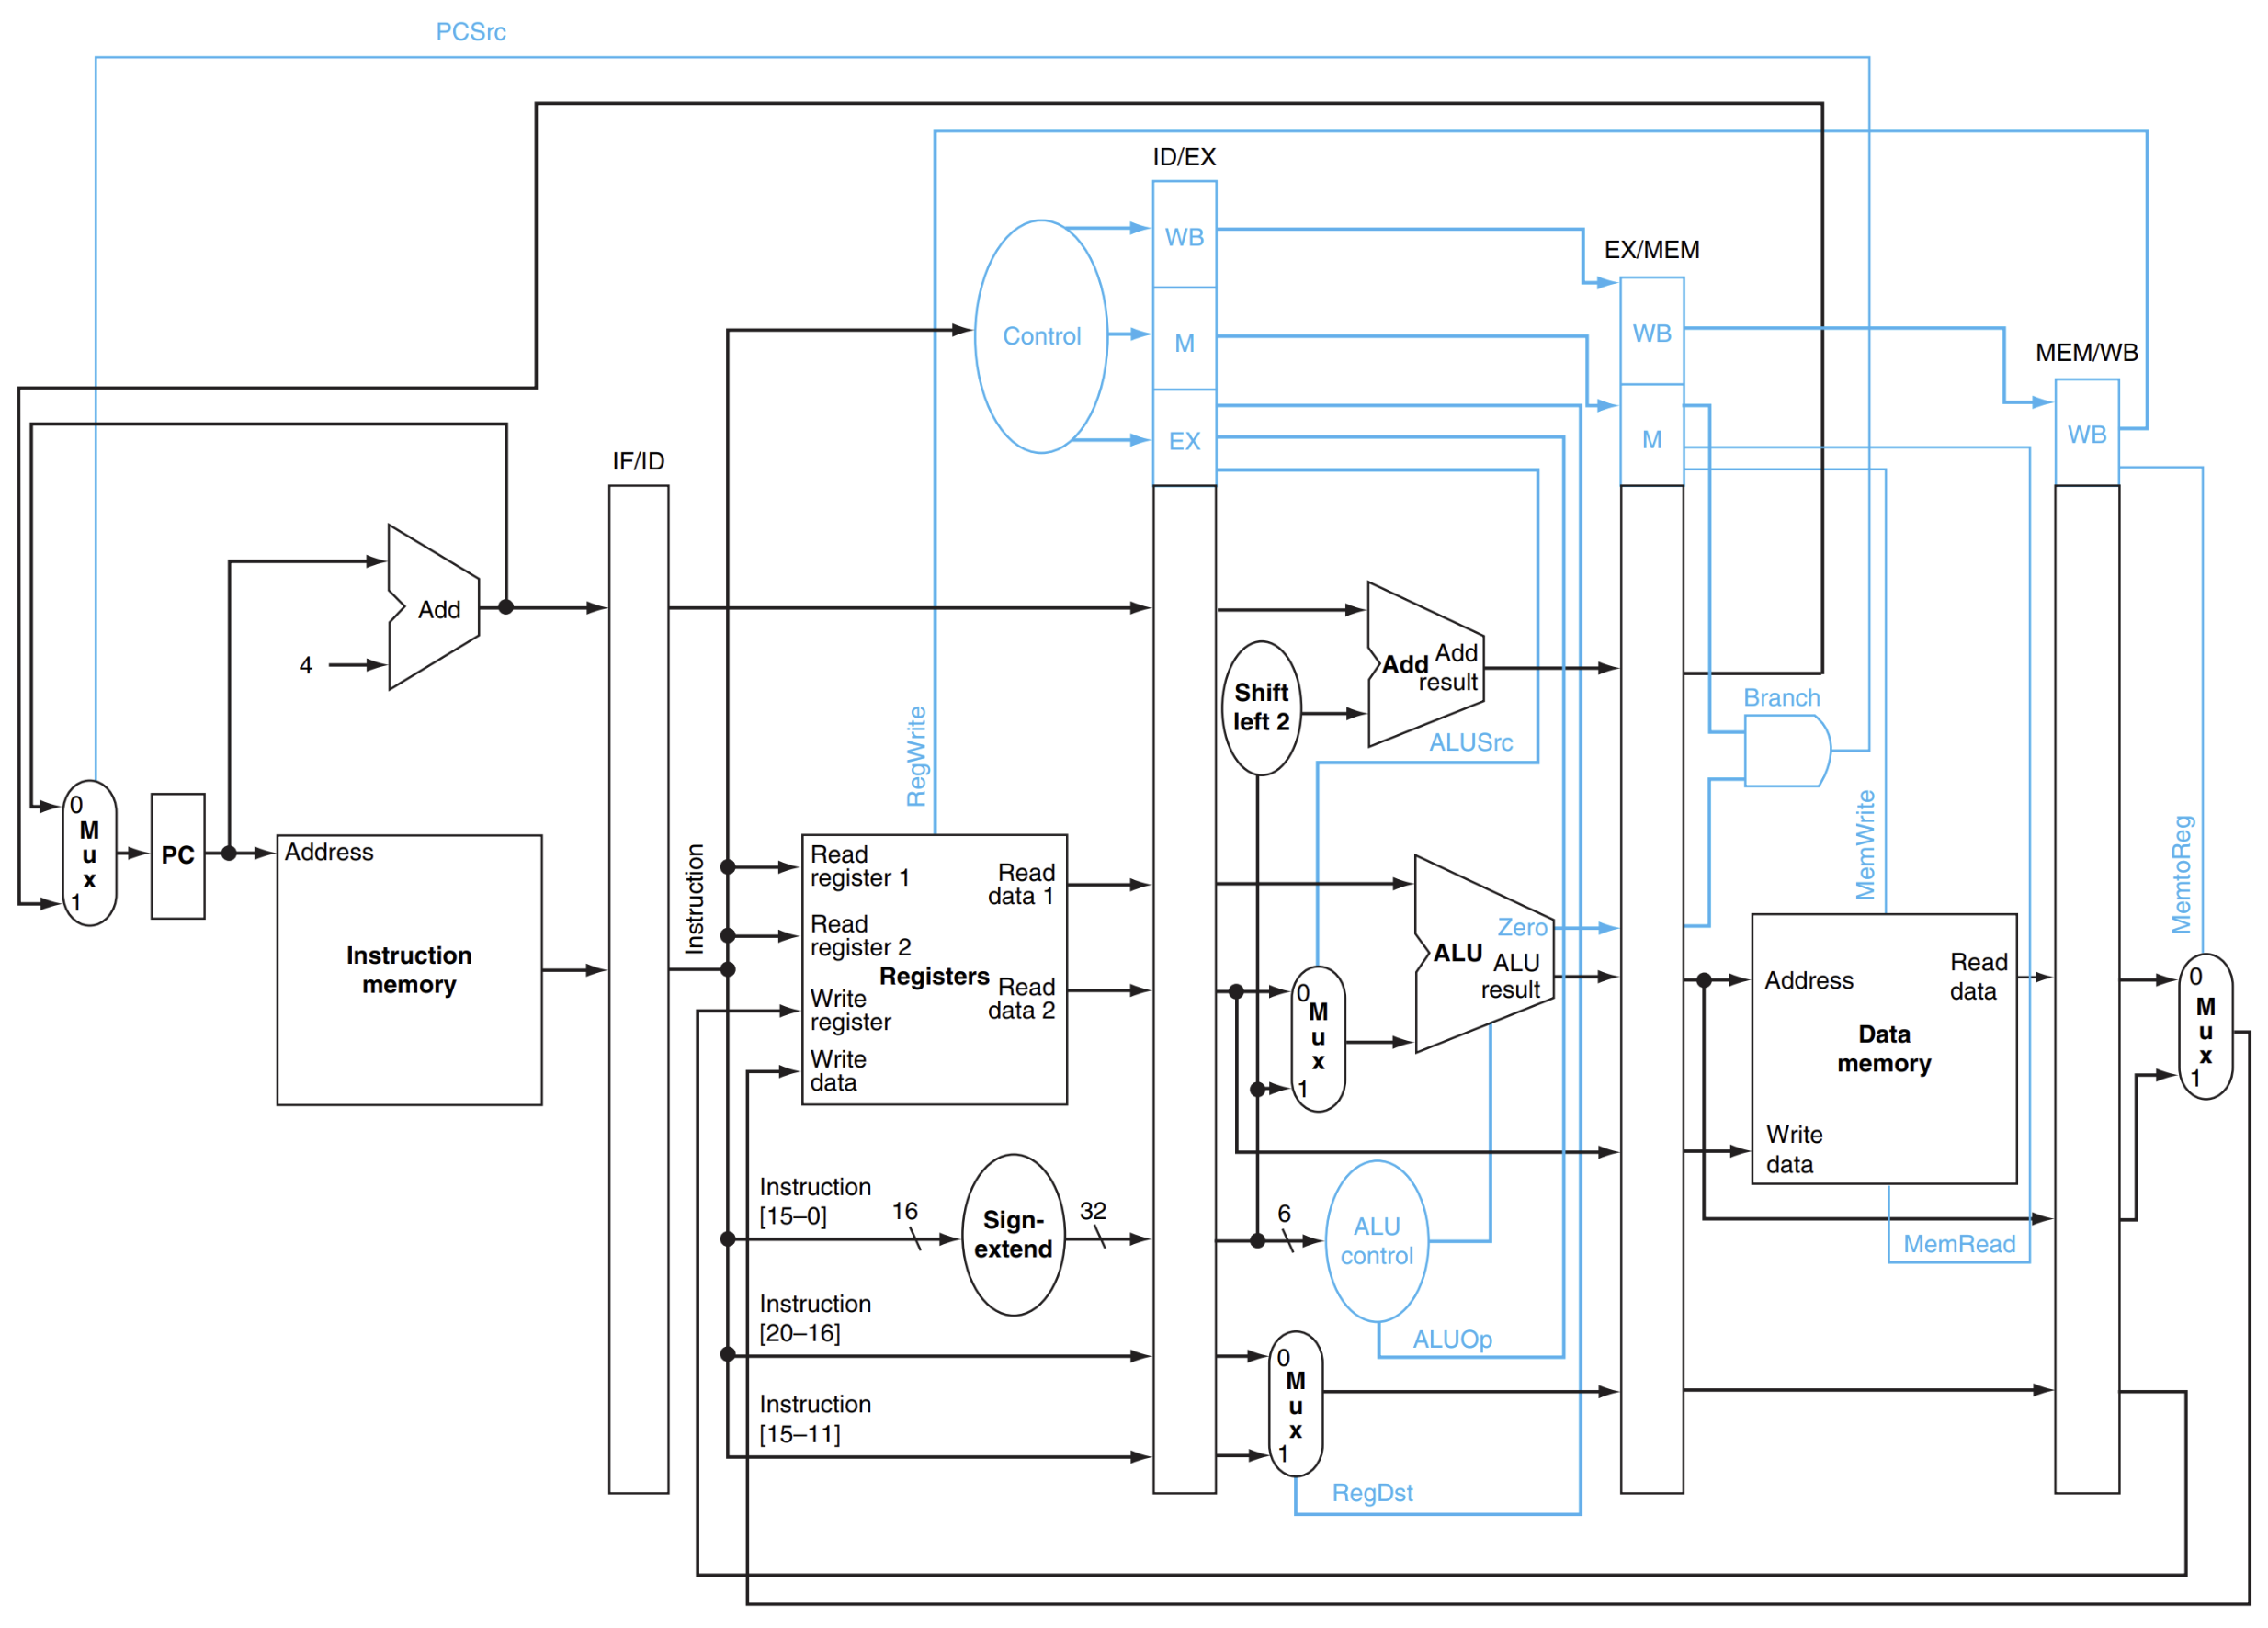
\includegraphics[width=1.0\textwidth]{cpu_big.jpg}
  \caption{MIPS Datapath with Interstage Registers.}
  \label{fig:cpu_big}
\end{figure}

\newpage

\paragraph{Exercise 1:} 
IF/ID: 
\begin{itemize}
    \item 32 bits for instruction
    \item 32 bits for PC
    \item Total = 64bits
    \item Minimum = 128 bits.
\end{itemize}
ID/EX:
\begin{itemize}
    \item 32 bits for instruction
    \item 32 bits for PC
    \item 32 bits for read data 1
    \item 32 bits for read data 2
    \item 3 bits for ALUOp
    \item 3 bits for MemWrite
    \item 2 bits for WriteBack
    \item 5 bits for RD
    \item 5 bits for RT
    \item Total = 146 bits
    \item Minimum = 256 bits
\end{itemize}
EX/MEM: 
\begin{itemize}
    \item 32 bits for instruction
    \item 32 bits for PC
    \item 32 bits for ALU result
    \item 2 bits for MemWrite
    \item 5 bits for RD
\end{itemize}
MEM/WB: 
\begin{itemize}
    \item 32 bits for instruction
    \item 32 bits for ALU result
    \item 32 bits for PC
    \item 2 bits for WriteBack
\end{itemize}
\newpage

\paragraph{Exercise 2. [10 Marks]} Consider a multi-core processor with 4 cores (named P1, P2, P3, P4), each with a dedicated cache. All 4 cores are attempting to read and write to the same cache block. The accesses to that cache block are serialized in the order that they are listed in the following table, from top to bottom.

Use the MESI protocol to complete the following table, showing the state of the cache block in each cache as requests are being processed. In each row, specify the state of the cache block in each core's cache after the request has been satisfied. On a cache miss, also specify all possible data suppliers. Assume that all caches are initially empty. Fill the following table (the first 3 lines are filled as a hint).

\begin{center}
\begin{tabular}{|c|c|c|c|c|c|c|}
\hline
\textbf{op} & \textbf{P1} & \textbf{P2} & \textbf{P3} & \textbf{P4} & \textbf{Supplier} \\
\hline
P1Read & E & - & - & - & Main Mem \\
\hline
P1Write & M & - & - & - & None \\
\hline
P2Read & S & S & - & - & P1 \\
\hline
P3Write & I & I & M & - & None \\
\hline
P1Read & S & I & S & - & P3 \\
\hline
P4Read & S & I & S & S & P1 or P3 \\
\hline
P3Read & S & I & S & S & None \\
\hline
P2Read & S & S & S & S & P1, P3, or P4 \\
\hline
P3Write & I & I & M & I & None\\
\hline
P4Write & I & I & I & M & None \\
\hline
P2Read & I & S & I & S & P4 \\
\hline
P4Write & I & I & I & M & None \\
\hline
\end{tabular}
\end{center}

\newpage

\paragraph{Exercise 3. [10 Marks]} Consider the following C code segment where \textit{a} and \textit{b} are 32-bit integer arrays of size \textit{n}.
\begin{verbatim}
    for (int i = 0; i < n; ++i) {
        int t = a[i];
        a[i] = b[i];
        b[i] = t + 2;
    }
\end{verbatim}

We have a corresponding MIPS instruction sequence, where \$s0, \$s1, \$s2, and \$t4 initially store, respectively, the base address of \textit{a}, the base address of \textit{b}, \textit{n}, and \textit{i} = 0.

\begin{verbatim}
    loop:
        lw   $t1, 0($s0)
        lw   $t2, 0($s1)
        sw   $t2, 0($s0)
        addi $t1, $t1, 2
        sw   $t1, 0($s1)
        addi $s0, $s0, 4
        addi $s1, $s1, 4
        addi $t4, $t4, 1
        slt  $t5, $t4, $s2
        bne  $t5, $0, loop
\end{verbatim}

Assume that the above MIPS instructions will be executed on a 5-stage pipelined processor. Ignore control hazards and structural hazard. Assume the branch condition is computed in the EX stage.

\begin{enumerate}
    \item [(a)]
    Draw the pipeline execution diagram (see \textit{L13-HazardExamples.pdf}) for one iteration of the loop: from the first \texttt{lw}, up to and including the \texttt{bne}. Assume there is no data forwarding. Do not re-order the instructions.

    Answer: The table is too large to fit in, so it is put in next page, (EX3. a)in the landscape mode.
  
    \item[(b)] 
    Now, assume all possible data forwarding is used. Draw the pipeline execution diagram for one iteration of the loop: from the first \texttt{lw}, up to and including the \texttt{bne}. For each instance of data forwarding annotate your pipeline diagram (say, with arrows, colors, and/or footnotes) to indicate the source and destination of the forwarding; also say what kind of forwarding it is. Do not re-order the instructions.

    Answer: This one is also too big to fit in. Check the next page for the table. (EX3. b)

    \item[(c)] 
    Apply loop unrolling (as well as instruction re-ordering, if you like) on the MIPS code segment so that the unrolled code is equivalent to two iterations of the original. Write out your final MIPS instruction code. Make sure to use offsets appropriately to avoid unnecessary instructions. You may assume \textit{n} is a multiple of 2.

    Answer:
    \begin{verbatim}
      loop:
      lw   $t1, 0($s0)
      lw   $t2, 0($s1)
      lw   $t3, 4($s0)
      lw   $t4, 4($s1)
      sw   $t2, 0($s0)
      sw   $t4, 4($s1)
      addi $t1, $t1, 2
      addi $t3, $t3, 2
      sw   $t1, 4($s0)
      sw   $t3, 8($s1)
      addi $s0, $s0, 8
      addi $s1, $s1, 8
      addi $t4, $t4, 2
      addi $t5, $t5, 2
      slt  $t6, $t5, $s2
      bne  $t6, $0, loop
    \end{verbatim}

    \item[(d)] 
    Consider a 2-issue extension of MIPS. That is, a VLIW extension of MIPS where two instructions occur in each issue packet. The issue packet has the following format: the first instruction must be arithmetic or branch, and the second instruction must be a data transfer instruction (\texttt{lw} or \texttt{sw}). Still assume all types of forwarding.

    Using the code of your unrolled loop of part (c), statically schedule one iteration of the (now unrolled) loop to run optimally on this 2-issue machine. You may wish to modify your code from part (c) to have a different order and use additional registers to accomplish this task. Consider using the following table as a starting point and to help guide you through the process

    \begin{center}
      \begin{tabular}{|c|c|c|c|}
      \hline
       & ALU or branch & Data transfer & CC \\
      \hline
      loop: & addi t4, t4, 2 & lw   t1, 0(s0) & 1 \\
      \hline
            & addi t5, t5, 2 & lw   t2, 0(s1) & 2 \\
      \hline
            & addi t1, t1, 2 & sw   t2, 0(s0) & 3 \\
      \hline
            & addi t3, t3, 2 & lw   t3, 4(s0) & 4 \\
      \hline
            & sw   1, 4(s0) & lw   t4, 4(s1) & 5 \\
      \hline
            & addi s0, s0, 8 & sw   t3, 8(s1) & 6 \\
      \hline
            & addi s1, s1, 8 & & 7 \\
      \hline
            & slt  t6, t5, s2 & & 8 \\
      \hline
            & bne  t6, 0, loop & & 9 \\
      \hline
      \end{tabular}
      \end{center}
      
    \begin{sidewaystable}{(EX3. a)}
      \begin{tabular}{|c|*{23}{c|}}
      \hline
      Cycle & 1 & 2 & 3 & 4 & 5 & 6 & 7 & 8 & 9 & 10 & 11 & 12 & 13 & 14 & 15 & 16 & 17 & 18 & 19 & 20 & 21 & 22 & 23 \\
      \hline
      lw $t1, 0(s0)$ & IF & ID & EX & ME & WB & & & & & & & & & & & & & & & & & & \\
      \hline
      lw $t2, 0(s1)$ & & IF & ID & EX & ME & WB & & & & & & & & & & & & & & & & & \\
      \hline
      NOP & & & x & x & x & x & x & & & & & & & & & & & & & & & & \\
      \hline
      NOP & & & & x & x & x & x & x & & & & & & & & & & & & & & & \\
      \hline
      sw $t2, 0(s0)$ & & & & & IF & ID & EX & ME & & & & & & & & & & & & & & & \\
      \hline
      addi $t1, t1, 2$ & & & & & & IF & ID & EX & ME & WB & & & & & & & & & & & & & \\
      \hline
      NOP & & & & & & & x & x & x & x & x & & & & & & & & & & & & \\
      \hline
      NOP & & & & & & & & x & x & x & x & x & & & & & & & & & & & \\
      \hline
      sw $t1, 0(s1)$ & & & & & & & & & IF & ID & EX & ME & & & & & & & & & & & \\
      \hline
      addi $s0, s0, 4$ & & & & & & & & & & IF & ID & EX & ME & WB & & & & & & & & & \\
      \hline
      addi $s1, s1, 4$ & & & & & & & & & & & IF & ID & EX & ME & WB & & & & & & & & \\
      \hline
      addi $t4, t4, 1$ & & & & & & & & & & & & IF & ID & EX & ME & WB & & & & & & & \\
      \hline
      NOP & & & & & & & & & & & & & x & x & x & x & x & & & & & & \\
      \hline
      NOP & & & & & & & & & & & & & & x & x & x & x & x & & & & & \\
      \hline
      slt $t5, t4, s2$ & & & & & & & & & & & & & & & IF & ID & EX & ME & WB & & & & \\
      \hline
      NOP & & & & & & & & & & & & & & & & x & x & x & x & x & & & \\
      \hline
      NOP & & & & & & & & & & & & & & & & & x & x & x & x & x & & \\
      \hline
      bne $t5, 0, loop$ & & & & & & & & & & & & & & & & & & IF & ID & EX & ME & WB & \\
      \hline
      \end{tabular}
      \end{sidewaystable}
      
      \begin{sidewaystable}{(EX3. b)}
        \begin{tabular}{|c|*{23}{c|}}
        \hline
        Cycle & 1 & 2 & 3 & 4 & 5 & 6 & 7 & 8 & 9 & 10 & 11 & 12 & 13 & 14 & 15 & 16 & 17 & 18 & 19 & 20 & 21 & 22 & 23 \\
        \hline
        lw $t1, 0(s0)$ & IF & ID & \cellcolor{yellow}EX & ME & WB & & & & & & & & & & & & & & & & & & \\
        \hline
        lw $t2, 0(s1)$ & & IF & ID & \cellcolor{yellow}EX & ME & WB & & & & & & & & & & & & & & & & & \\
        \hline
        sw $t2, 0(s0)$ & & & IF & ID & \cellcolor{green}EX & ME & & & & & & & & & & & & & & & & & \\
        \hline
        addi $t1, t1, 2$ & & & & IF & ID & \cellcolor{green}EX & ME & WB & & & & & & & & & & & & & & & \\
        \hline
        sw $t1, 0(s1)$ & & & & & IF & ID & EX & ME & & & & & & & & & & & & & & & \\
        \hline
        addi $s0, s0, 4$ & & & & & & IF & ID & EX & ME & WB & & & & & & & & & & & & & \\
        \hline
        addi $s1, s1, 4$ & & & & & & & IF & ID & EX & ME & WB & & & & & & & & & & & & \\
        \hline
        addi $t4, t4, 1$ & & & & & & & & IF & ID & \cellcolor{red}EX & ME & WB & & & & & & & & & & & \\
        \hline
        slt $t5, t4, s2$ & & & & & & & & & IF & ID & \cellcolor{purple}EX & ME & WB & & & & & & & & & & \\
        \hline
        bne $t5, 0, loop$ & & & & & & & & & & IF & ID & \cellcolor{blue}EX & ME & WB & & & & & & & & & \\
        \hline
        \end{tabular}
        \end{sidewaystable}
      
\end{enumerate}

\newpage
\paragraph{Exercise 4. [10 Marks]}
Consider a multi-core processor with 2 cores, named P1 and P2.
Each core has a dedicated cache with the following characteristics:
\begin{itemize}
  \item 2-way set associative and a 16-byte capacity;
  \item is initially empty;
  \item follows the MESI snooping protocol;
  \item follows write-back and write-allocate protocols; and
  \item follows a pseudo-LRU replacement policy where
  \begin{enumerate}
    \item[(i)] empty cache lines in a set are filled first, then,
    \item[(ii)] if there are any invalid cache lines in a set replace them, then,
    \item[(iii)] if no invalid cache lines are present, follows a typical LRU replacement policy.
  \end{enumerate}
\end{itemize}
Given the following list of serialized memory byte address accesses by the cores, determine:
\begin{enumerate}
  \item[(a)] whether each access results in a cache hit, cold miss, conflict miss, capacity miss, true share miss, or false share miss;
  \item[(b)] the data stored in each cache after all addresses in the list have been accessed; and
  \item[(c)] the MESI state of each cache block after all addresses in the list have been accessed.
\end{enumerate}
 
\begin{center}
\begin{tabular}{|c|l|c||c|l|c|}
\hline
Time & Memory Access & Hit/Miss Type & Time & Memory Access & Hit/Miss Type \\
\hline
1 & P1 Reads 5 & cold & 11 & P2 Writes 9 & hit \\
\hline
2 & P2 Writes 8 & cold & 12 & P2 Writes 10 & cold \\
\hline
3 & P1 Reads 9 & cold & 13 & P2 Reads 2 & cold \\
\hline
4 & P1 Writes 14 & cold & 14 & P1 Writes 7 & cold \\
\hline
5 & P1 Reads 3 & cold & 15 & P1 Reads 8 & false \\
\hline
6 & P1 Writes 12 & cold & 16 & P1 Reads 4 & conflict \\
\hline
7 & P2 Reads 6 & cold & 17 & P2 Reads 12 & cold \\
\hline
8 & P2 Reads 17 & cold & 18 & P2 Reads 7 & true \\
\hline
9 & P1 Reads 20 & cold & 19 & P1 Writes 2 & hit \\
\hline
10 & P2 Reads 4 & cold & 20 & P1 Reads 11 & cold \\
\hline
\end{tabular}
\end{center}

\vspace{2em}

To answer part (a) use the above table. To answer parts (b) and (c), use the below tables.

\begin{center}
\begin{tabularx}{\textwidth}{|c|X|X|c||c|X|X|c|}
\hline
\multicolumn{4}{|c||}{P1 Cache} & \multicolumn{4}{c|}{P2 Cache} \\
\hline
Set & \multicolumn{2}{c|}{Cache Block Data} & State & Set & \multicolumn{2}{c|}{Cache Block Data}& State \\
\hline
\multirow{2}{*}{0} & 8 & 9 & S & \multirow{2}{*}{0} & 8 & 9 & S\\
\cline{2-4} \cline{6-8}
& & & & & 16& 17& E\\
\hline
\multirow{2}{*}{1} & 2 & 3 & M & \multirow{2}{*}{1} & 10 & 11 & S\\
\cline{2-4} \cline{6-8}
& 10& 11& S& & 2& 3& I\\
\hline
\multirow{2}{*}{2} & 20& 21& E& \multirow{2}{*}{2} & 4& 5& S\\
\cline{2-4} \cline{6-8}
& 4& 5& S& & 12& 13& E\\
\hline
\multirow{2}{*}{3} & 14& 15& M& \multirow{2}{*}{3} & 6& 7& S\\
\cline{2-4} \cline{6-8}
& 6& 7& S& & & & \\
\hline
\end{tabularx}
\end{center}
\end{document}
